\documentclass[11pt]{article}
\usepackage[a4paper,margin=25mm]{geometry}
\usepackage{amsmath,amssymb,amsthm,mathtools,bm}
\usepackage{booktabs,array,microtype,graphicx}
\usepackage[hidelinks]{hyperref}
\usepackage[nameinlink,noabbrev]{cleveref}
\hypersetup{
  pdftitle={Algebraic Query Support for Unitary Oracles},
  pdfauthor={Lluis Eriksson},
  pdfsubject={Fixed-trace unitary discrimination and oracle-variety query ranks},
  pdfkeywords={quantum query complexity, unitary discrimination, Hilbert function, spherical harmonics}
}

\newtheorem{theorem}{Theorem}[section]
\newtheorem{proposition}[theorem]{Proposition}
\newtheorem{corollary}[theorem]{Corollary}
\newtheorem{lemma}[theorem]{Lemma}
\theoremstyle{definition}
\newtheorem{definition}[theorem]{Definition}
\theoremstyle{remark}
\newtheorem{remark}[theorem]{Remark}

\newcommand{\C}{\mathbb C}
\newcommand{\PP}{\mathbb P}
\newcommand{\Span}{\operatorname{span}}
\newcommand{\rank}{\operatorname{rank}}
\newcommand{\Tr}{\operatorname{Tr}}
\newcommand{\Sym}{\operatorname{Sym}}
\newcommand{\cH}{\mathcal H}
\newcommand{\cV}{\mathcal V}
\newcommand{\cF}{\mathcal F}
\newcommand{\ket}[1]{\lvert #1\rangle}
\newcommand{\bra}[1]{\langle #1\rvert}
\newcommand{\vket}[1]{\lvert #1\rangle\!\rangle}
\newcommand{\vbra}[1]{\langle\!\langle #1\rvert}

\title{\textbf{Algebraic Query Support for Unitary Oracles}\\
Exact Hilbert Laws, Harmonic Spectra, and General-Tester Bounds}
\author{Lluis Eriksson}
\date{August 2026}

\begin{document}
\maketitle

\begin{abstract}
The usual dimension bound for discrimination with $k$ calls to a $d$-level
unitary oracle is the ambient symmetric-tensor count
$\binom{k+d^2-1}{k}$.  It ignores polynomial relations satisfied by a
restricted oracle family.  We show that the exact linear support exposed by
$k$ forward calls is instead the degree-$k$ Hilbert function of the
projective Zariski closure of that family.  Every causally ordered $k$-query
protocol consequently obeys a Hilbert-rank discrimination bound.

For the noncentral, nontraceless fixed-angle qubit class
$U(\bm n)=qI-ir\bm n\cdot\bm\sigma$, $\bm n\in S^2$, $qr\neq0$, this gives the exact
quadratic law $H_X(k)=(k+1)^2$, rather than the unrestricted cubic count
$\binom{k+3}{3}$.  At the traceless endpoint the rank is
$\binom{k+2}{2}$, while a central class has rank one.  We use the transitive
orbit average and its constant leverage score to
prove the stronger operational statement
\[
 P_{\rm succ}^{\rm GEN}\leq \min\{1,D_k/M\}
\]
for every uniform $M$-hypothesis subset and every general tester.  Thus the
fixed-angle promise refines the unrestricted general-tester numerator
$\binom{k+3}{3}$ to $D_k=(k+1)^2$.  Beyond qubits, a selective phase
oracle on an unknown ray in $\C^d$ has projective closure equal to a linearly
transformed Segre variety.  Its exact support is
$\binom{k+d-1}{d-1}^{\!2}$: the ambient degree $d^2-1$ collapses to $2d-2$,
and the two-query defect is $d^2(d-1)^2/4$.
We then diagonalize the
continuous $k$-copy Bell frame exactly: its eigenvalues are finite
Funk--Hecke sums indexed by spherical harmonics of ranks $0\leq\ell\leq k$.
This yields an exact purity and a participation dimension that grows only
linearly in $k$, despite quadratic algebraic support.  We prove that the
continuous frame is tight in the interior only for one query at $q^2=1/4$;
it is never tight there for $k\geq2$.  Spherical $2k$-designs inherit the same spectrum.
Great-circle oracles form a conic subfamily with exact rank $2k+1$ and a
closed Fourier spectrum.  The results separate support rank, effective rank,
and operational attainability.  They do not assert that every full-rank
ensemble attains the dimension bound or that every general process matrix has
a laboratory realization.
\end{abstract}

\section{Introduction}

A $k$-query circuit can only create amplitudes that are homogeneous
polynomials of degree $k$ in the entries of its oracle.  The polynomial method
is foundational in quantum query complexity~\cite{beals2001,sheyuen2023}.  In unitary
channel discrimination, an analogous ambient count gives the general bound
$\binom{k+d^2-1}{k}/M$ for $M$ equiprobable $d$-dimensional unitary
hypotheses~\cite{bavaresco2022}.  That count is optimal without structural
information about the oracle set.  It is not intrinsic to a constrained
family.

The missing datum is the homogeneous ideal of the oracle family.  If the
allowed projective matrices lie on an algebraic variety $X$, every equation
in $I(X)$ removes a symmetric-tensor direction.  The surviving number of
directions is exactly the Hilbert function $H_X(k)$~\cite{eisenbud1995}.  This observation turns
the ambient polynomial method into a geometry-sensitive query bound.

Our main application is physically elementary but structurally nontrivial.
Fix the eigenphases of an $SU(2)$ gate and vary only its rotation axis:
\begin{equation}\label{eq:class}
 U(\bm n)=e^{-i\theta\bm n\cdot\bm\sigma/2}
 =qI-ir\,\bm n\cdot\bm\sigma,
 \quad q=\cos(\theta/2),\quad r=\sin(\theta/2),\quad \bm n\in S^2.
\end{equation}
Here $q,r\in\mathbb R$, $q^2+r^2=1$, and $\Tr U=2q$.  Although channel
representatives have an arbitrary global phase, the promise itself is the
phase-invariant quantity $|\Tr U|^2/4=q^2$; the displayed representatives
fix the $SU(2)$ convention.  Physically, the sphere describes a pulse with
known rotation angle and unknown field axis.  This is a conjugacy class of
fixed-angle qubit rotations, a family also
appearing in quantum learning of rotations about an unknown
direction~\cite{mochiribella2019}.  Its nondegenerate projective closure is a
quadric surface, so its $k$-query support grows as $(k+1)^2$.  The result
sharpens the unrestricted qubit count by
\begin{equation}\label{eq:deficitintro}
 \binom{k+3}{3}-(k+1)^2=\binom{k+1}{3}.
\end{equation}
At two queries this is a one-dimensional defect; at general $k$ it is a
cubic cumulative deficit.

The contributions are:
\begin{enumerate}
\item an oracle-variety theorem identifying exact causal query support with a
Hilbert function, together with uniform and nonuniform causal bounds;
\item the complete three-branch rank law for fixed-angle qubit rotations and
the exact rank law for a great-circle restriction;
\item an arbitrary-dimension law for rank-one selective-phase oracles, whose
Segre geometry changes the ambient support exponent from $d^2-1$ to $2d-2$;
\item a transitive-orbit leverage theorem refining the ultimate general-tester
bound of Bavaresco--Murao--Quintino from $\binom{k+3}{3}/M$ to
$D_k/M$ on the fixed-angle class;
\item a finite closed formula for every eigenvalue of the continuous
$k$-copy frame, including endpoint cascades, exact purity, and effective rank;
\item a sharp obstruction showing that one-query tightness does not persist
at any interior angle for $k\geq2$;
\item an exact positive-scalability criterion that distinguishes a dimension
upper bound from its attainability by a fixed effective state family.
\end{enumerate}

The harmonic analysis, Hilbert functions, leverage inequality, and spherical
designs used below are classical~\cite{seeley1966,delsarte1977}.  The claimed
contribution is their exact synthesis with algebraic quantum-query support
and general-tester discrimination.  We do not claim new general theory of
spherical harmonics, algebraic varieties, or process matrices.

Dimensional and linear-independence bounds for repeated gate identification
are direct antecedents~\cite{chefles2007,chiribella2013}.  Likewise, the
orbit-average domination mechanism is classical in covariant quantum
estimation~\cite{chiribella2006} and appears explicitly in the ultimate
general-tester proof of \cite[Appendix F]{bavaresco2022}.  Our new claim is
therefore the exact promise-class numerator, its singular branch diagram, and
the accompanying all-$k$ harmonic spectra---not a new tester formalism or a
first orbit-domination lemma.

She and Yuen's generalized polynomial method shows that a $T$-query unitary
property test has an acceptance polynomial of degree at most $2T$ and uses
invariant theory to derive property-testing lower bounds~\cite{sheyuen2023}.
Our statement is complementary: it concerns the exact pure-state span of
$k$ forward calls, uses the full homogeneous ideal rather than an invariant
acceptance polynomial, and feeds that span into finite-ensemble channel
discrimination.  We do not claim to originate the unitary polynomial method.

The $k=2$ identity $10\to9$ was previously isolated for a specific
24-echo tetrahedral ensemble, together with a causal saturation certificate,
in~\cite{eriksson2026echo}.  Here it is one instance of an all-$k$ law for
arbitrary fixed-angle subsets.  The present work additionally treats the
three singular branches, compact-orbit general testers, exact continuous
spectra, and the planar-axis restriction; it does not reuse the special
tetrahedral attainment certificate.

\begin{table}[t]
\centering
\small
\caption{Priority boundary: classical mechanisms versus the consequences
derived here.}
\label{tab:priority}
\begin{tabular}{@{}p{0.22\textwidth}p{0.34\textwidth}p{0.37\textwidth}@{}}
\toprule
Source & Established mechanism & Present use or additional conclusion \\
\midrule
Beals et al.; She--Yuen & Query amplitudes/acceptance probabilities are
low-degree polynomials; invariant theory yields property-testing bounds. &
The full oracle ideal gives the exact pure-state support $H_X(k)$ and a
finite-ensemble rank converse. \\
Bavaresco et al. & Ambient symmetric-tensor domination for general testers. &
The orbit numerator is replaced by the exact promise rank $D_k$, including
all singular branches. \\
Funk--Hecke and spherical designs & Harmonic diagonalization and exact
cubature for polynomial kernels. & Exact fixed-angle spectra, purity,
endpoint cascades, and the all-$k$ tightness obstruction. \\
Segre geometry & Rank-one matrices have coordinate space
$H^0(\mathcal O(k,k))$. & Selective-phase qudit oracles acquire support
$\binom{k+d-1}{d-1}^2$ and a GEN discrimination cap. \\
\bottomrule
\end{tabular}
\end{table}

\section{Forward-query model and projective oracle families}

Let $V$ be a finite-dimensional complex vector space containing the matrix
entries of an oracle.  A unitary channel is unchanged by multiplying its
implementing matrix by a global phase, so oracle matrices naturally determine
points of $\PP(V)$.  Let $\mathcal U\subset\PP(V)$ be a family of projective
unitary matrices and let $X=\overline{\mathcal U}^{\,Z}$ denote its complex
projective Zariski closure.  Write
\begin{equation}
 H_X(k)=\dim_\C\bigl(\C[V]/I(X)\bigr)_k
\end{equation}
for its degree-$k$ Hilbert function.

We use the standard forward-oracle model: each query inserts the same unknown
unitary $U$, not $U^\dagger$ and not a controlled version of an otherwise
uncontrolled black box.  Arbitrary known isometries, ancillas, coherent
feedback, and intermediate measurements are allowed.  Intermediate
measurements can be deferred after adding a record system.

We also use the general-tester model of
Bavaresco--Murao--Quintino~\cite{bavaresco2022}.  For a $d$-level unitary let
\begin{equation}
 \vket{U}=(I\otimes U)\sum_{a=0}^{d-1}\ket a\ket a,
 \qquad J_U=\vket{U}\vbra{U} .
\end{equation}
Thus $\Tr J_U=d$ and $\Tr_OJ_U=I$.  A general $k$-copy tester is a family
$T_i\geq0$ whose deterministic sum $W=\sum_iT_i$ obeys
\begin{equation}\label{eq:generaltester}
 \Tr\!\left[W(C_1\otimes\cdots\otimes C_k)\right]=1
\end{equation}
for every tuple of channel Choi operators $C_1,\ldots,C_k$.  This feasible
class contains parallel and causally ordered testers and is the mathematical
general-process class used in that reference.  We do not assume that every
element has a laboratory realization.

\begin{lemma}[Multilinear normal form]\label{lem:normalform}
For every purified causally ordered circuit making $k$ forward calls to $U$,
there is a fixed linear map $L$, independent of $U$, such that its final pure
state satisfies
\begin{equation}
 \ket{\Psi_U}=L\,U^{\otimes k}.
\end{equation}
Tensor-factor permutations, fixed input vectors, ancillary identities, and
all intermediate isometries are absorbed into $L$.
\end{lemma}

\begin{proof}
Expand the circuit in fixed bases.  Every path amplitude contains exactly one
matrix entry from each oracle call and hence is a homogeneous degree-$k$
polynomial in the entries of $U$.  Collecting its coefficients defines $L$.
Purifying every known channel and coherently storing every measurement outcome
reduces the general causal circuit to this case without changing the best
final discrimination probability.
\end{proof}

\section{The oracle-variety query law}

\begin{theorem}[Hilbert query-support law]\label{thm:hilbert}
For every $k\geq0$,
\begin{equation}\label{eq:hilbertspan}
 \dim\!\left(\Span\{U^{\otimes k}:[U]\in\mathcal U\}\right)=H_X(k).
\end{equation}
Consequently, the final states of every purified causal $k$-query circuit have
linear span of dimension at most $H_X(k)$.
\end{theorem}

\begin{proof}
The Veronese vector $U^{\otimes k}$ belongs to $\Sym^k(V)$.  Its annihilator
inside $\Sym^k(V)^*$ consists exactly of homogeneous degree-$k$ polynomials
that vanish on $\mathcal U$.  Polynomial vanishing is unchanged by Zariski
closure, so the annihilator is $I(X)_k$.  Rank--nullity gives
\begin{equation}
 \dim\!\left(\Span\{U^{\otimes k}\}\right)
 =\dim\Sym^k(V)-\dim I(X)_k=H_X(k).
\end{equation}
The circuit statement follows from \cref{lem:normalform} because a fixed
linear map cannot increase span dimension.
\end{proof}

The support value in \cref{thm:hilbert} is operationally exposed by a causal
parallel architecture: feed the $k$ calls with $k$ Bell pairs.  The resulting
pure vector is $\vket{U}^{\otimes k}$, and vectorization is injective, so its
hypothesis span has dimension exactly $H_X(k)$.  Thus $H_X(k)$ is the maximum
causal support, not merely an upper bound on it.

\begin{corollary}[Causal discrimination bounds]\label{cor:causalbound}
Let $U_1,\ldots,U_M\in\mathcal U$ have priors $p_i$.  Every causal $k$-query
protocol satisfies
\begin{equation}\label{eq:priorbound}
 P_{\rm succ}\leq
 \min\{1,p_{\max}H_X(k)\},\qquad p_{\max}=\max_i p_i.
\end{equation}
For uniform priors this becomes
$P_{\rm succ}\leq\min\{1,H_X(k)/M\}$.
\end{corollary}

\begin{proof}
Let $P$ project onto the span of the purified final hypothesis vectors and let
$\{M_i\}$ be the final POVM.  Since
$\ket{\Psi_i}\!\bra{\Psi_i}\leq P$,
\begin{align}
 P_{\rm succ}
 &=\sum_i p_i\Tr\!\left(M_i\ket{\Psi_i}\!\bra{\Psi_i}\right)\\
 &\leq p_{\max}\sum_i\Tr(PM_iP)
 =p_{\max}\Tr P\leq p_{\max}H_X(k).
\end{align}
\end{proof}

If $X$ has positive projective dimension $s$ and degree $\Delta$, its Hilbert
polynomial gives
\begin{equation}\label{eq:hilbertasymptotic}
 H_X(k)=\frac{\Delta}{s!}k^s+O(k^{s-1}).
\end{equation}
Thus the geometry of the oracle family fixes the exponent of accessible
support.  A necessary asymptotic condition for perfect identification of $M$
generic hypotheses is
$k\gtrsim(s!M/\Delta)^{1/s}$.  It is only necessary: positivity and the
geometry of the finite ensemble can impose further obstructions.

\begin{remark}[Relation to the polynomial method]
The fact that query amplitudes are low-degree polynomials is classical in
Boolean-oracle complexity~\cite{beals2001}.  \Cref{thm:hilbert} identifies the
exact quotient dimension after imposing the homogeneous ideal of a continuous
matrix-oracle family.  For $X=\PP^{d^2-1}$ it reduces to the ambient count
$\binom{k+d^2-1}{k}$ used in the general unitary discrimination
bound~\cite{bavaresco2022}.
\end{remark}

\section{Transitive orbits: an ultimate general-tester bound}

The Hilbert law above applies to arbitrary projective oracle families but is
proved through causal circuit amplitudes.  Transitive unitary orbits admit a
stronger statement because their leverage score is constant.

\begin{lemma}[Compact-orbit leverage]\label{lem:leverage}
Let a compact group act transitively on a unitary orbit $\{U_x:x\in\Omega\}$,
with invariant probability measure $\mu$.  Set
\begin{equation}
 v_x=\vket{U_x}^{\otimes k},\qquad
 \overline J_k=\int_\Omega \ket{v_x}\bra{v_x}\,d\mu(x),\qquad
 D_k=\rank\overline J_k.
\end{equation}
Then, for every $x$,
\begin{equation}\label{eq:rankonedomination}
 \ket{v_x}\bra{v_x}\leq D_k\,\overline J_k.
\end{equation}
The constant $D_k$ is the smallest orbit-independent constant for which this
operator inequality holds.
\end{lemma}

\begin{proof}
The orbit representation is unitary, so $\overline J_k$ and its
Moore--Penrose inverse commute with it.  Hence
$L(x)=\langle v_x|\overline J_k^+|v_x\rangle$ is constant.  Averaging gives
\begin{equation}
 L(x)=\Tr(\overline J_k^+\overline J_k)=D_k.
\end{equation}
For $A\geq0$ and $v\in\operatorname{ran}A$, Cauchy--Schwarz applied to
$A^{+1/2}v$ gives
$\ket v\bra v\leq\langle v|A^+|v\rangle A$.  This proves
\cref{eq:rankonedomination}.  Applying $\langle v_x|\overline J_k^+(\cdot)
\overline J_k^+|v_x\rangle$ to any uniform domination shows that its constant
cannot be smaller than $D_k$.
\end{proof}

\begin{theorem}[Ultimate bound on a transitive unitary orbit]
\label{thm:genbound}
Let $U_1,\ldots,U_M$ be any finite subset of a compact transitive unitary
orbit and suppose the labels are equiprobable.  Every general $k$-copy tester
satisfies
\begin{equation}\label{eq:genbound}
 P_{\rm succ}^{\rm GEN}\leq\min\left\{1,\frac{D_k}{M}\right\}.
\end{equation}
For arbitrary priors, the safe variant is
$P_{\rm succ}^{\rm GEN}\leq\min\{1,p_{\max}D_k\}$.
\end{theorem}

\begin{proof}
Write $J_i=J_{U_i}$ and $W=\sum_iT_i$.  By
\cref{lem:leverage}, $J_i^{\otimes k}\leq D_k\overline J_k$.  Positivity and
\cref{eq:generaltester} give
\begin{align}
 P_{\rm succ}
 &=\frac1M\sum_i\Tr(T_iJ_i^{\otimes k})\\
 &\leq\frac{D_k}{M}\Tr(W\overline J_k)
 =\frac{D_k}{M},
\end{align}
because $\Tr(WJ_{U_x}^{\otimes k})=1$ for every $x$ and hence also after
averaging.  Replacing each prior by $p_{\max}$ proves the nonuniform bound.
\end{proof}

When $D_k\leq M$, equality at $D_k/M$ is not automatic.  With
$A_i=D_k\overline J_k-J_i^{\otimes k}\geq0$, it holds for a given tester if
and only if $\Tr(T_iA_i)=0$ for every $i$.  If $P$ projects onto
$\operatorname{ran}\overline J_k$, this forces
\begin{equation}\label{eq:reciprocaltester}
 PT_iP=c_i\ket{\overline J_k^+v_i}\bra{\overline J_k^+v_i},
 \qquad c_i\geq0,
\end{equation}
together with the deterministic-tester normalization.  Thus full orbit span
is necessary but not sufficient for attaining the cap.

\section{Fixed-angle qubit rotations: three exact branches}

In the Pauli basis, \cref{eq:class} has projective coordinates
$[x_0:x_1:x_2:x_3]=[q:-irn_1:-irn_2:-irn_3]$.

\begin{theorem}[Fixed-angle rank law]\label{thm:ranklaw}
For $k\geq1$, define
\begin{equation}
 \cV_k(q,r)=\Span_\C\{U(\bm n)^{\otimes k}:\bm n\in S^2\}.
\end{equation}
Then
\begin{equation}\label{eq:ranklaw}
 \dim\cV_k(q,r)=
 \begin{cases}
 (k+1)^2,&qr\neq0,\\[2mm]
 \binom{k+2}{2},&q=0,\ r\neq0,\\[2mm]
 1,&r=0.
 \end{cases}
\end{equation}
For $qr\neq0$, generic $M$ axes have finite-ensemble rank
$\min\{M,(k+1)^2\}$.
\end{theorem}

\begin{proof}
When $qr\neq0$, the projective closure is the smooth quadric
\begin{equation}\label{eq:quadric}
 x_1^2+x_2^2+x_3^2=-\frac{r^2}{q^2}x_0^2\subset\PP^3.
\end{equation}
Its Hilbert series is $(1-t^2)/(1-t)^4$, whose degree-$k$ coefficient is
\begin{equation}
 \binom{k+3}{3}-\binom{k+1}{3}=(k+1)^2.
\end{equation}
Equivalently, the feature blocks are all symmetric monomials in $\bm n$ of
degrees $0,\ldots,k$.  Fischer decomposition identifies their restrictions
to the sphere with
$\bigoplus_{\ell=0}^k\cH_\ell$, of total dimension
$\sum_{\ell=0}^k(2\ell+1)=(k+1)^2$.

If $q=0$, only the homogeneous degree-$k$ feature remains.  The tensors
$\bm n^{\otimes k}$ span $\Sym^k(\C^3)$: a homogeneous polynomial vanishing
on the real unit sphere vanishes on every nonzero real vector by scaling and
therefore vanishes identically.  The dimension is $\binom{k+2}{2}$.  If
$r=0$, the class contains one projective oracle.  Finally, because the full
evaluation span has the displayed finite dimension, some set of that many
axes is independent; nonvanishing of an evaluation minor is Zariski open,
which proves the generic finite-set statement.
\end{proof}

At the traceless endpoint $U(-\bm n)=-U(\bm n)$, so antipodal axes implement
the same unitary channel.  The physical promise space is therefore
$\mathbb{RP}^2$, not a sphere of distinct channel labels.  Counting both
$\bm n$ and $-\bm n$ as different hypotheses would introduce an unavoidable
label ambiguity and cannot lead to perfect channel identification.

\begin{corollary}[Ultimate fixed-angle query bound]\label{cor:querylower}
For $M$ equiprobable fixed-angle qubit hypotheses with $qr\neq0$,
\begin{equation}
 P_{\rm succ}^{\rm GEN}(k)\leq
 \min\left\{1,\frac{(k+1)^2}{M}\right\}.
\end{equation}
Perfect identification requires
$k\geq\lceil\sqrt M\rceil-1$.  At $q=0$ it instead requires
$\binom{k+2}{2}\geq M$.
\end{corollary}

\begin{proof}
The $SU(2)$ conjugation action is transitive on the fixed-angle sphere, so
\cref{thm:genbound} applies with the ranks in \cref{thm:ranklaw}.  The query
conditions follow by requiring the relevant numerator to be at least $M$.
They are necessary, not sufficient.
\end{proof}

\begin{table}[t]
\centering
\caption{Exact $k$-query support dimensions for the indicated qubit oracle
families and singular branches.}
\label{tab:ranks}
\begin{tabular}{@{}lll@{}}
\toprule
Oracle geometry & defining structure & support dimension \\
\midrule
unrestricted projective matrices & $\PP^3$ & $\binom{k+3}{3}$ \\
fixed angle, $qr\neq0$ & quadric surface & $(k+1)^2$ \\
traceless fixed angle & homogeneous sphere features & $\binom{k+2}{2}$ \\
fixed-angle great circle & plane conic & $2k+1$ \\
traceless great circle & homogeneous binary features & $k+1$ \\
central class & one point & $1$ \\
\bottomrule
\end{tabular}
\end{table}

\begin{figure}[t]
\centering
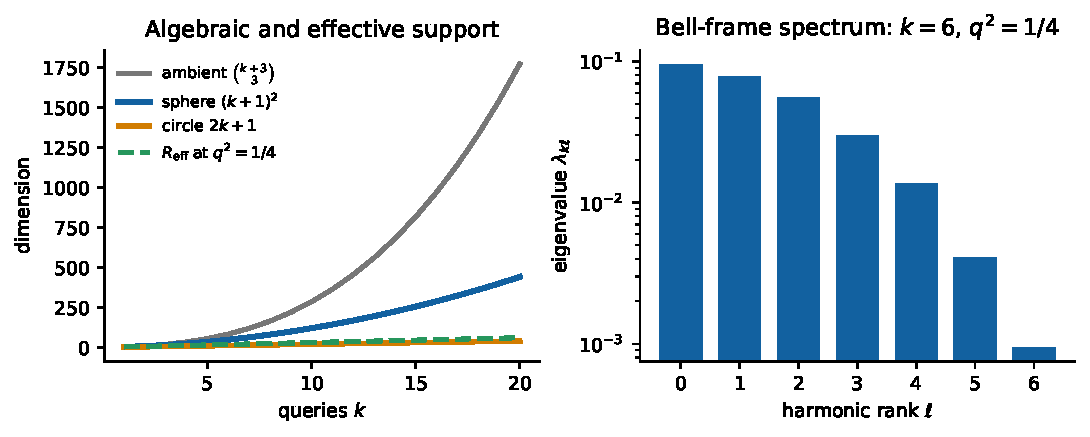
\includegraphics[width=\textwidth]{oracle_variety_spectrum.pdf}
\caption{Left: unrestricted, fixed-sphere, and fixed-circle query dimensions,
 together with the Bell-frame effective rank at $q^2=1/4$.  The fixed-angle
promise changes the general-tester numerator from cubic to quadratic, while a
planar-axis promise makes it linear.  Right: the exact harmonic
eigenvalues at $k=6$ illustrate why effective and algebraic ranks differ.}
\label{fig:rankspectrum}
\end{figure}

\section{Rank-one phase oracles in arbitrary dimension}

The qubit quadric is the first member of a higher-dimensional family with a
more dramatic support reduction.  Let $d\geq2$, let $\ket\psi\in\C^d$ be an
unknown unit vector, and consider the selective phase oracle
\begin{equation}\label{eq:phaseoracle}
 U_\psi=I+cP_\psi,\qquad
 P_\psi=\ket\psi\!\bra\psi,\qquad c=e^{i\vartheta}-1.
\end{equation}
It applies the known phase $e^{i\vartheta}$ to one unknown ray and acts as the
identity on its orthogonal complement.  The promise is transitive under
unitary conjugation.

\begin{theorem}[Segre query-support law]\label{thm:segre}
For $k\geq1$, set
\begin{equation}
 D_{d,k}(c)=\dim\Span\{U_\psi^{\otimes k}:\ket\psi\in\C^d,\ \|\psi\|=1\}.
\end{equation}
Then
\begin{equation}\label{eq:segrerank}
 D_{d,k}(c)=
 \begin{cases}
 1,&c=0,\\[1mm]
 \binom{k+2}{2},&d=2,\ c=-2,\\[2mm]
 \binom{k+d-1}{d-1}^{\!2},&\text{otherwise}.
 \end{cases}
\end{equation}
On the generic branch the support exponent is $2d-2$, rather than the
unrestricted matrix exponent $d^2-1$.
\end{theorem}

\begin{proof}
Projective rank-one matrices form the Segre variety
\begin{equation}
 \Sigma_d=\PP^{d-1}\times(\PP^{d-1})^*\hookrightarrow\PP(\operatorname{End}\C^d).
\end{equation}
The physical projectors are Zariski dense in $\Sigma_d$: equivalently, the
$U(d)$ orbit complexifies to the dense $GL_d$ orbit of rank-one matrices with
nonzero trace.  Define the linear map
\begin{equation}
 L_c(X)=\Tr(X)I+cX.
\end{equation}
For $\Tr P_\psi=1$, one has $L_c(P_\psi)=U_\psi$.  On the scalar and traceless
summands of $\operatorname{End}\C^d$, the eigenvalues of $L_c$ are respectively
$c+d$ and $c$.  Hence $L_c$ is invertible unless $c=0$ or $c=-d$.

When it is invertible, the projective oracle closure is a linear image of
$\Sigma_d$.  Its degree-$k$ coordinate space is
\begin{equation}
 H^0(\Sigma_d,\mathcal O(k,k))
 \cong \Sym^k(\C^d)^*\otimes\Sym^k(\C^d),
\end{equation}
of dimension $\binom{k+d-1}{d-1}^2$.  The Hilbert query-support law now gives
the last line of \cref{eq:segrerank}.

For a unit-modulus phase, $c=-d$ can occur only when $d=2$ and $c=-2$.
Then $L_c$ kills the scalar coordinate and sends the Bloch projectors onto
the projective traceless space $\PP^2$, whose Hilbert function is
$\binom{k+2}{2}$.  Finally, $c=0$ makes every oracle equal to $I$.
\end{proof}

\begin{corollary}[Qudit phase-oracle discrimination]\label{cor:segregen}
For $M$ equiprobable hypotheses from the orbit in \cref{eq:phaseoracle}, every
general $k$-copy tester obeys
\begin{equation}
 P_{\rm succ}^{\rm GEN}\leq\min\{1,D_{d,k}(c)/M\}.
\end{equation}
On the generic branch, perfect identification therefore requires
\begin{equation}
 \binom{k+d-1}{d-1}^{\!2}\geq M.
\end{equation}
At two queries the exact reduction from the unrestricted support is
\begin{equation}\label{eq:quditdefect}
 \binom{d^2+1}{2}-\binom{d+1}{2}^{\!2}
 =\frac{d^2(d-1)^2}{4}.
\end{equation}
Thus the qutrit support is $36$ rather than $45$, and the four-level support
is $100$ rather than $136$.
\end{corollary}

\begin{proof}
The orbit is compact and transitive, so \cref{thm:genbound} applies with
\cref{thm:segre}.  Equation~\eqref{eq:quditdefect} is an elementary
simplification of the two displayed dimensions.
\end{proof}

For fixed $d$ and large $k$, the generic support satisfies
\begin{equation}
 D_{d,k}(c)=\frac{k^{2d-2}}{((d-1)!)^2}+O(k^{2d-3}),
\end{equation}
whereas the unrestricted support is
$k^{d^2-1}/(d^2-1)!+O(k^{d^2-2})$.  The promise therefore changes not only a
constant but the polynomial growth exponent.  When $d=2$, the generic Segre
law reduces to $(k+1)^2$, and its exceptional phase $c=-2$ is exactly the
traceless branch of \cref{thm:ranklaw}.

\section{When is a support bound attained?}

Rank alone does not construct a tester.  The following statement concerns a
fixed family of effective pure states, after the query architecture has been
chosen; it is not an existence theorem for a causal architecture.

\begin{theorem}[Fixed-state scalability criterion]\label{thm:scalability}
Let $\ket{\phi_i}$ be normalized vectors with Gram matrix $K$, common span
projector $P$, and rank $D$.  For uniform priors, their dimension bound $D/M$
is attained if and only if there are weights $c_i\geq0$ such that
\begin{equation}\label{eq:scalable}
 \sum_i c_i\ket{\phi_i}\!\bra{\phi_i}=P.
\end{equation}
Equivalently, for $C=\operatorname{diag}(c_i)$,
\begin{equation}\label{eq:kck}
 KCK=K.
\end{equation}
In that case $\sum_i c_i=D$ and
$M_i=c_i\ket{\phi_i}\!\bra{\phi_i}$ is an attaining POVM on the support.
\end{theorem}

\begin{proof}
The estimate
$\Tr(M_i\ket{\phi_i}\!\bra{\phi_i})\leq\Tr(PM_iP)$
is an equality only if the compressed positive operator $PM_iP$ is supported
on $\C\phi_i$.  Equality in the sum therefore forces
$PM_iP=c_i\ket{\phi_i}\!\bra{\phi_i}$ and POVM completeness gives
\cref{eq:scalable}.  Conversely, \cref{eq:scalable} supplies a POVM with
success $M^{-1}\sum_i c_i=D/M$.  Multiplying the frame identity by the
analysis and synthesis maps gives \cref{eq:kck}; the reverse implication
holds on the frame range.  Taking the trace gives $\sum_i c_i=D$.
\end{proof}

This criterion isolates three logically different resources: algebraic
support $D$, the ability of a circuit to realize useful vectors inside that
support, and positive scalability of those vectors.  A full-rank evaluation
table need not satisfy the last condition.

\section{Exact harmonic spectrum of the continuous class}

Use normalized one-query Bell/Choi vectors
\begin{equation}
 \ket{u_{\bm n}}=q\ket0-ir\sum_{a=1}^3n_a\ket a,
 \qquad
 \langle u_{\bm n}|u_{\bm m}\rangle=a+b\,\bm n\cdot\bm m,
\end{equation}
where $a=q^2$, $b=r^2$, and $a+b=1$.  Define the continuous $k$-copy frame
operator
\begin{equation}\label{eq:frame}
 F_k=\int_{S^2}
 \ket{u_{\bm n}}\!\bra{u_{\bm n}}^{\otimes k}\,d\omega(\bm n),
\end{equation}
with normalized area measure.

\begin{theorem}[Funk--Hecke spectrum]\label{thm:spectrum}
If $ab>0$, the nonzero eigenvalues of $F_k$ are
\begin{equation}\label{eq:lambdaspectrum}
 \lambda_{k\ell}^{\times(2\ell+1)},\qquad 0\leq\ell\leq k,
\end{equation}
where
\begin{align}
 \lambda_{k\ell}
 &=\frac12\int_{-1}^{1}(a+bx)^kP_\ell(x)\,dx\label{eq:funkhecke}\\
 &=\sum_{\substack{\ell\leq j\leq k\\j-\ell\ {\rm even}}}
 \binom{k}{j}a^{k-j}b^j
 \frac{j!}{(j-\ell)!!(j+\ell+1)!!}.\label{eq:finitespectrum}
\end{align}
Every displayed eigenvalue is positive and
$\sum_{\ell=0}^k(2\ell+1)\lambda_{k\ell}=1$.
At $a=0$, exactly the sectors $\ell\equiv k\pmod2$ survive.
\end{theorem}

\begin{proof}
The integral operator with the same nonzero spectrum as $F_k$ has zonal
kernel $(a+b\bm n\cdot\bm m)^k$.  Funk--Hecke diagonalizes it on each
spherical harmonic space $\cH_\ell$ and gives \cref{eq:funkhecke}.  Expanding
the binomial and using
\begin{equation}
 \frac12\int_{-1}^1x^jP_\ell(x)\,dx
 =\frac{j!}{(j-\ell)!!(j+\ell+1)!!}
\end{equation}
when $j\geq\ell$ has the same parity as $\ell$, and zero otherwise, proves
\cref{eq:finitespectrum}.  The $j=\ell$ term proves positivity for $ab>0$.
The trace identity follows by evaluating the kernel on the diagonal.
\end{proof}

\begin{proposition}[Exact purity and effective rank]\label{prop:purity}
For $b>0$,
\begin{equation}\label{eq:purity}
 \Tr F_k^2=
 \frac{1-(a-b)^{2k+1}}{2b(2k+1)},
 \qquad
 R_{\rm eff}(F_k)=
 \frac{2b(2k+1)}{1-(a-b)^{2k+1}}.
\end{equation}
For every fixed interior angle, $R_{\rm eff}(F_k)=2b(2k+1)+o(1)$ as
$k\to\infty$, whereas $\rank F_k=(k+1)^2$.
\end{proposition}

\begin{proof}
Using two independent axes and rotational invariance,
\begin{align}
 \Tr F_k^2
 &=\int\!\!\int
 |\langle u_{\bm n}|u_{\bm m}\rangle|^{2k}
 d\omega(\bm n)d\omega(\bm m)\\
 &=\frac12\int_{-1}^{1}(a+bx)^{2k}\,dx,
\end{align}
which integrates to \cref{eq:purity}, since $a+b=1$.  For $0<a,b<1$ one
has $|a-b|<1$, giving the asymptotic statement.
\end{proof}

Thus algebraic support and participation dimension have different scaling:
the former is quadratic and the latter linear.  The exact frame entropy is
also immediately available as
\begin{equation}
 S(F_k)=-\sum_{\ell=0}^k(2\ell+1)
 \lambda_{k\ell}\log\lambda_{k\ell},
\end{equation}
but no entropy optimality is asserted here.

\subsection{Endpoint cascades}

The rank jumps in \cref{eq:ranklaw} are resolved spectrally.  As $b\downarrow0$,
\begin{equation}\label{eq:centralcascade}
 \lambda_{k\ell}=
 \frac{k!}{(k-\ell)!(2\ell+1)!!}
 a^{k-\ell}b^\ell+O(b^{\ell+1}),
\end{equation}
so angular sectors disappear successively with harmonic rank.  As
$a\downarrow0$, sectors with $k-\ell$ even have nonzero limits
\begin{equation}
 \lambda_{k\ell}\longrightarrow
 \frac{k!}{(k-\ell)!!(k+\ell+1)!!},
\end{equation}
whereas opposite-parity sectors vanish at least linearly in $a=q^2$.
More precisely, when $k-\ell$ is odd,
\begin{equation}\label{eq:tracelesscascade}
 \lambda_{k\ell}=
 \frac{k!}{(k-\ell-1)!!(k+\ell)!!}\,a+O(a^2).
\end{equation}
Exactly $k(k+1)/2$ dimensions disappear at the traceless endpoint.

\section{Interior tightness is a one-query phenomenon}

\begin{theorem}[Sharp interior tightness obstruction]\label{thm:notight}
For $ab>0$, the continuous frame $F_k$ is tight on its support if and only if
$k=1$ and $a=q^2=1/4$.  In particular, it is never tight for any
$k\geq2$ at an interior fixed angle.
\end{theorem}

\begin{proof}
For $k=1$, \cref{eq:finitespectrum} gives
$\lambda_{10}=a$ and $\lambda_{11}=b/3$, so equality holds exactly at
$a=1/4$.  Let $k\geq2$.  Equality of the top two harmonic eigenvalues would
force
\begin{equation}
 \frac{\lambda_{k,k-1}}{\lambda_{k,k}}
 =(2k+1)\frac ab=1.
\end{equation}
At the resulting ratio $a/b=1/(2k+1)$, direct evaluation of the next sector
gives
\begin{equation}
 \frac{\lambda_{k,k-2}}{\lambda_{k,k}}
 =\frac{2k+1}{2}\left[1+(2k-1)(a/b)^2\right]
 =\frac{k(2k+3)}{2k+1}>1.
\end{equation}
The three sectors therefore cannot share one eigenvalue.
\end{proof}

At the traceless endpoint $a=0$, the one-query frame is tight on its
three-dimensional support, while for $k\geq2$ its surviving sectors already
have unequal top eigenvalues because
$\lambda_{k,k-2}/\lambda_{k,k}=(2k+1)/2\neq1$.  At the central endpoint
$a=1$ the frame has rank one and is trivially tight for every $k$.  These
endpoint statements are separate from the interior theorem.

\begin{corollary}[No positive reweighting restores Bell tightness]
\label{cor:noreweight}
For $ab>0$ and $k\geq2$, no finite nonzero positive measure on the full fixed-angle orbit
can make the $k$-copy Bell vectors a tight frame on their complete
$(k+1)^2$-dimensional span.
\end{corollary}

\begin{proof}
Let $P_\ell$ project onto the harmonic sector $\cH_\ell$.  Transitivity makes
$\|P_\ell u_{\bm n}^{\otimes k}\|^2$ independent of $\bm n$; its value is
$(2\ell+1)\lambda_{k\ell}$.  Therefore every positive weighted frame of total
mass $w$ has sector trace $w(2\ell+1)\lambda_{k\ell}$.  A scalar multiple of
the full support projector would instead have sector trace proportional to
$2\ell+1$, forcing all $\lambda_{k\ell}$ to coincide.
\Cref{thm:notight} excludes this for $k\geq2$.
\end{proof}

\begin{corollary}[Transfer to spherical designs]\label{cor:design}
If a finite weighted axis set is a spherical $2k$-design, its discrete
$k$-copy Bell frame equals $F_k$ and has exactly the spectrum in
\cref{thm:spectrum}.  Hence no such equal-weight frame is tight for
$k\geq2$ at an interior angle.
\end{corollary}

\begin{proof}
Every matrix entry of the frame integrand is a polynomial of total degree at
most $2k$ in the axis coordinates.  The design identity therefore replaces
the integral exactly by the finite weighted sum.
\end{proof}

The corollary does not say that every design is a transitive group orbit, nor
that no alternative query input can attain the general-tester dimension cap.

\section{Planar-axis oracles: conic rank and Fourier spectrum}

Restrict the axis to
$\bm n(\varphi)=(\cos\varphi,\sin\varphi,0)$.  The projective closure is a
plane conic.  This is a control promise in which the unknown field axis is
known a priori to lie in a plane (two available quadratures), rather than a
separate physical memory resource.

\begin{theorem}[Great-circle law]\label{thm:circle}
For $ab>0$,
\begin{equation}
 \dim\!\left(\Span\{U(\bm n(\varphi))^{\otimes k}:\varphi\in[0,2\pi)\}\right)=2k+1.
\end{equation}
The continuous frame has Fourier eigenvalues
\begin{equation}\label{eq:circleeig}
 \mu_{km}=
 \sum_{\substack{|m|\leq j\leq k\\j-m\ {\rm even}}}
 \binom{k}{j}a^{k-j}b^j2^{-j}
 \binom{j}{(j-m)/2},
 \qquad -k\leq m\leq k.
\end{equation}
All are positive.  At $a=0$, only modes $m\equiv k\pmod2$ survive and the
rank becomes $k+1$.
\end{theorem}

\begin{proof}
The kernel is $(a+b\cos(\varphi-\psi))^k$.  Its Fourier support is contained
in $-k,\ldots,k$, and the $j=|m|$ term is nonzero when $ab>0$, proving exact
rank $2k+1$.  Expanding $\cos^j\theta=2^{-j}(e^{i\theta}+e^{-i\theta})^j$
gives \cref{eq:circleeig}.  If $a=0$, only $j=k$ remains.
\end{proof}

At $a=0$, antipodal points again differ only by global phase, so the physical
channel family is $\mathbb{RP}^1$.  Distinct-hypothesis counts must quotient
this identification before applying a perfect-discrimination criterion.

Because rotations around the normal act transitively on the circle,
\cref{thm:genbound} also gives
\begin{equation}
 P_{\rm succ}^{\rm GEN,circ}\leq
 \begin{cases}
 \min\{1,(2k+1)/M\},&ab>0,\\
 \min\{1,(k+1)/M\},&a=0,\\
 1/M,&b=0.
 \end{cases}
\end{equation}

The circle is an explicit warning against inferring support dimension from
the number of continuous parameters alone: both the sphere and the circle
are infinite families, but their Hilbert functions are respectively
quadratic and linear.

\section{Operational consequences and comparisons}

For nondegenerate fixed-angle qubit oracles, the accessible support hierarchy
is
\begin{equation}
 \underbrace{R_{\rm eff}(F_k)}_{\Theta(k)}
 \ \leq\ 
 \underbrace{\rank F_k}_{(k+1)^2}
 \ \leq\ 
 \underbrace{\binom{k+3}{3}}_{\text{unrestricted ambient}}.
\end{equation}
Each quantity answers a different question.  The first measures spectral
participation of one canonical continuous Bell encoding; the second is the
maximum algebraic support exposed by the oracle family; the third ignores the
fixed-angle relation.

For example, $M=24$ generic fixed-angle hypotheses cannot be perfectly
identified with fewer than four forward queries, because
$(k+1)^2<24$ for $k\leq3$.  This is a necessary query lower bound, not a
four-query construction.  At $k=2$, the family-specific support cap is
$9/M$, whereas the unrestricted qubit cap is $10/M$.  The all-$k$ deficit in
\cref{eq:deficitintro} shows that this is the first member of a growing
sequence rather than an isolated accident.  The earlier tetrahedral-echo
paper~\cite{eriksson2026echo} proves this $k=2$ defect for one nontransitive
24-label ensemble and, crucially, certifies causal attainment there.  The
present result generalizes the support defect to all $k$ and arbitrary
fixed-angle subsets, extends the bound to the transitive-orbit GEN class, and
adds the singular branch laws and exact sphere/circle spectra; it makes no
new claim about that ensemble's adaptive certificate.

More sharply, the class-to-ambient ratio is
\begin{equation}
 \frac{(k+1)^2}{\binom{k+3}{3}}
 =\frac{6(k+1)}{(k+2)(k+3)}\sim\frac6k.
\end{equation}
Thus the promise removes an asymptotically dominant fraction of the ambient
query space, not merely a fixed finite defect.

The contrast with the unrestricted result is operational, not merely a rank
calculation.  Bavaresco--Murao--Quintino prove the ambient
$\binom{k+3}{3}/M$ cap for general qubit testers~\cite{bavaresco2022};
\cref{thm:genbound} replaces its numerator by the exact coordinate-ring rank
of the transitive fixed-angle promise.  For the full sphere the reduction is
$\binom{k+1}{3}$ dimensions, while the circle promise reduces the numerator
further to $2k+1$.

The higher-dimensional selective-phase family shows that the mechanism is
not peculiar to a quadric surface.  Its Segre closure changes the support
growth from $\Theta(k^{d^2-1})$ to $\Theta(k^{2d-2})$.  For fixed $d$, the
corresponding necessary query scale for $M$ generic labels drops from the
ambient degree count to
$k\gtrsim((d-1)!^2M)^{1/(2d-2)}$; this remains a converse, not a universal
attaining construction.

Fixed-angle rotation learning~\cite{mochiribella2019} studies a different
task: a direction is encoded in a spin system and later used to implement a
target rotation.  The present task is minimum-error identification from
repeated black-box gate calls.  The common conjugacy-class geometry explains
the shared use of $SU(2)$ covariance, but neither result implies the other.

\section{Reproducibility and scope}

The accompanying exact-arithmetic verifier checks, for a configurable range
of $k$, the Hilbert-rank identities, every rational Funk--Hecke eigenvalue at
rational $a$, trace and purity, endpoint ranks, great-circle Fourier
coefficients, and the tightness obstruction.  It is a finite symbolic audit,
not a computer proof of the general theorems.

The scope is deliberately precise:
\begin{itemize}
\item the Hilbert-function support identity is a causal forward-query theorem
for arbitrary projective families; the stronger general-tester cap is proved
only for compact transitive unitary orbits by constant leverage;
\item the general-tester class is the mathematical optimization class of
\cite{bavaresco2022}; no claim is made that every general process matrix is
physically realizable;
\item support rank is not automatically an achievable success probability;
\cref{thm:scalability} is a criterion for a fixed effective state family, not
a universal circuit synthesis theorem;
\item the continuous spectrum concerns the Bell/Choi parallel frame; it does
not optimize all inputs or all adaptive circuits;
\item spherical harmonics, Funk--Hecke theory, Hilbert functions, and
spherical designs are classical ingredients, as is the rank-one leverage
inequality;
\item controlled-$U$, calls to $U^\dagger$, postselection, and different
oracle models require new feature spaces and are not covered;
\item no noise robustness, experimental resource count, or asymptotic
statistical estimation theorem is inferred from exact algebraic rank.
\end{itemize}

\paragraph{AI assistance.}
OpenAI Codex assisted with symbolic exploration, literature triage, drafting,
and reproducibility checks.  The author is responsible for the definitions,
proofs, claims, citations, and final manuscript.

\section{Conclusion}

Quantum query support is controlled by the algebraic geometry of the oracle
family, not only by the size of its ambient matrix space.  The degree-$k$
Hilbert function gives the exact exposed dimension and therefore a direct
causal discrimination bound.  On a compact transitive orbit, constant
leverage upgrades the same rank to an ultimate general-tester cap.
Fixed-angle qubit rotations provide a complete case study: quadratic generic
support, a separate traceless branch, exact harmonic and Fourier spectra,
linear participation rank, and a sharp failure of multi-query Bell
tightness.  Rank-one phase oracles show in arbitrary dimension that the same
framework can reduce the ambient support exponent from $d^2-1$ to $2d-2$.
The resulting separation between ambient rank, promise-variety
rank, spectral participation, and operational attainability supplies a
portable framework for other constrained unitary orbits.

{\small
\bibliographystyle{unsrt}
\bibliography{references}
}

\end{document}
